\subsection{设计相关内容}
\subsubsection{理论要点}
\begin{itemize}
    \item[1)] 多周期CPU理论知识,包括控制器和数据通路,取址、译码、执行、回写等多个阶段。
    \item[2)] SOC顶层框架搭建的基本知识
    \item[3)] VGA、PS2等外部I/O接口的扩展知识
    \item[3)] MIPS汇编程序设计的理论知识,包括32条指令的实现细节,以及如何用现有指令合成伪指令的方式。
    \item[4)] 软硬件协同设计的基本思想
\end{itemize}

\subsubsection{技术工具}
\begin{itemize}
    \item[1)] 代码编辑器——VSCode
    \item[2)] soc框架工程搭建工具——ISE14.7
    \item[2)] 将mips转化为coe文件的汇编器mipsasm
    \item[3)] 执行coe文件的模拟器ZJUQS-II.SWORD.Emulator.v1.2.3
\end{itemize}

\subsubsection{设计方法}
自顶向下设计思想\\

\subsection{设计方案}
\subsubsection{物体位置信息的存放}
这里主要围绕如何存储实时更新变化的障碍物、坦克和子弹的话题给出一个解决方案。\\

在mips编程规范中,.data可以用于自定义标签和该标签上存放的内容,同样也支持数组的使用。因此这里可以将障碍物、坦克和子弹的位置信息存储在数组里,并在每次刷新屏幕的时候,遍历数组取出这些位置信息并更新。那么问题来了,怎么判别哪个地址段上的数据属于坦克,哪段数据又属于障碍物?为了解决这个问题,还需要额外设计一个num变量,用于存放当前障碍物的个数信息。此时如果要删除或插入一条新的记录,则可以根据num来遍历障碍物数组的所有数据,并进行整体的挪动或更新。\\

\begin{figure}[H]
  \centering
  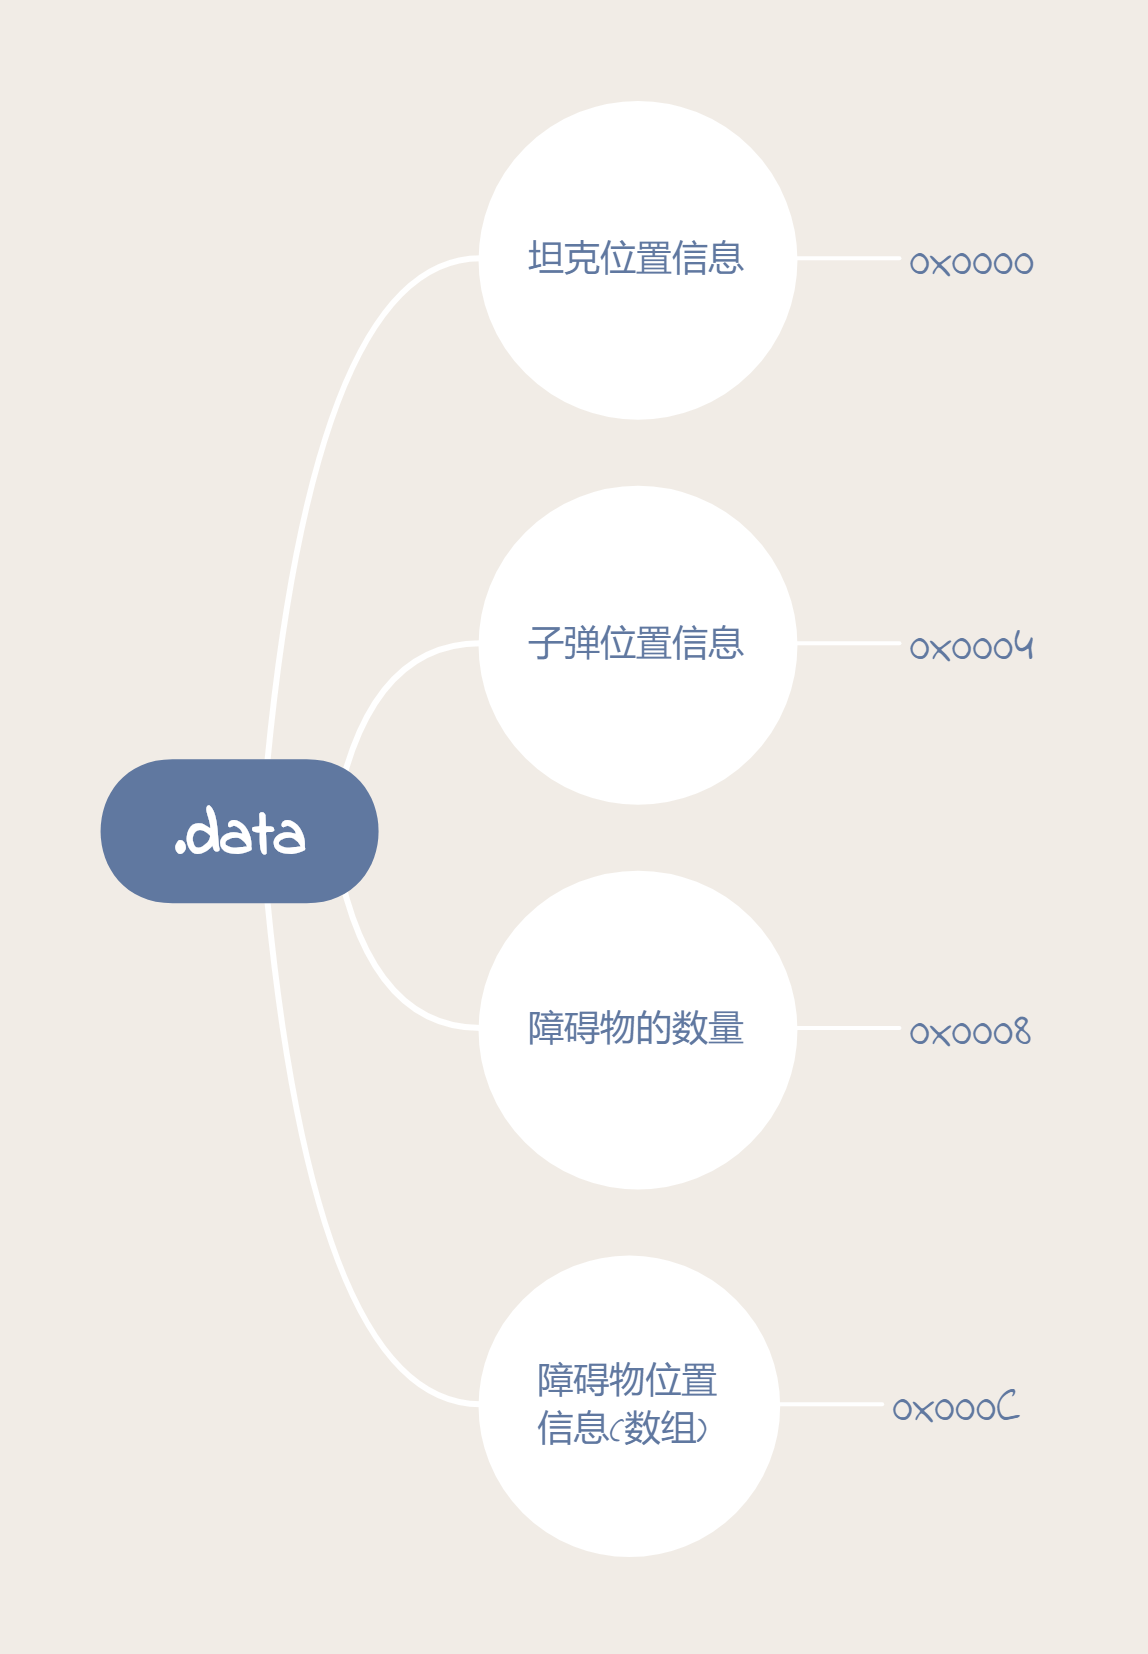
\includegraphics[width=0.5\textwidth]{img/data.png}
  \caption{.data标签及数据分配示意图
  }\label{fig:data}
\end{figure}

最后还有个问题,当.data里设计完指定的标签后,我们通常是用la \$rt, label这条伪指令将label所表示的地址值赋值给\$rt寄存器的,然而我所设计的多周期CPU并不支持这样一条伪指令。实际上,深入了解la指令之后可以发现,我们完全可以用addi \$rt, \$rs, address指令事先计算出label的值,然后再用lw \$rt, \$rs来获取label标记地址上的信息。此时,物体位置信息存放的问题就有了一个初步的解决方案。\\

\subsubsection{生成障碍物}
程序需要每隔一段时间在随机位置生成障碍物。实际上,我们不可能采取系统的主频来作为生成频率,那会导致障碍物生成过快,从而很快挤满屏幕。\\

为了解决这个问题,这里用\$t9寄存器作为障碍物生成的时间间隔变量,作为flag, 当\$t9=0x20000时生成新的障碍物,并且将flag \$t9重新置为0。这里采用这个数字作为flag的计时上限,是因为它是我经过多次参数的调整从而得到的一个比较合适的数字。一开始平均1s-2s生成新的障碍物,当障碍物数量多起来之后,需要调用的判断函数随之增加,flag递增的速度也会随之降低。因此可以获得,障碍物数量少的时候生成的速度快,障碍物数量多的时候生成的速度慢的效果,可以使玩家获得较好的体验感。

\subsubsection{随机坐标的获取}
随机坐标通过读写GPIO端口的counter计数器得到,并将其转化为符合640的x轴范围,480的y轴范围的坐标。再进一步通过绘制函数显示在屏幕上。

\subsection{硬件设计}
硬件设计部分参照多周期MCPU的实验报告,具体内容待返校物理验证后填写。

\subsection{系统软件设计}
这一部分将详细介绍"Only One Shot"汇编代码的设计细节,为了方便阅读,部分代码分析与解读直接放在注释里。

\subsubsection{模块概览}
为了便于理解,我将本项目的函数模块化,并绘制了对应的思维导图,从下图中可以看出各个模块之间的相互调用关系,以及整个程序运行的流程。

\begin{figure}[H]
  \centering
  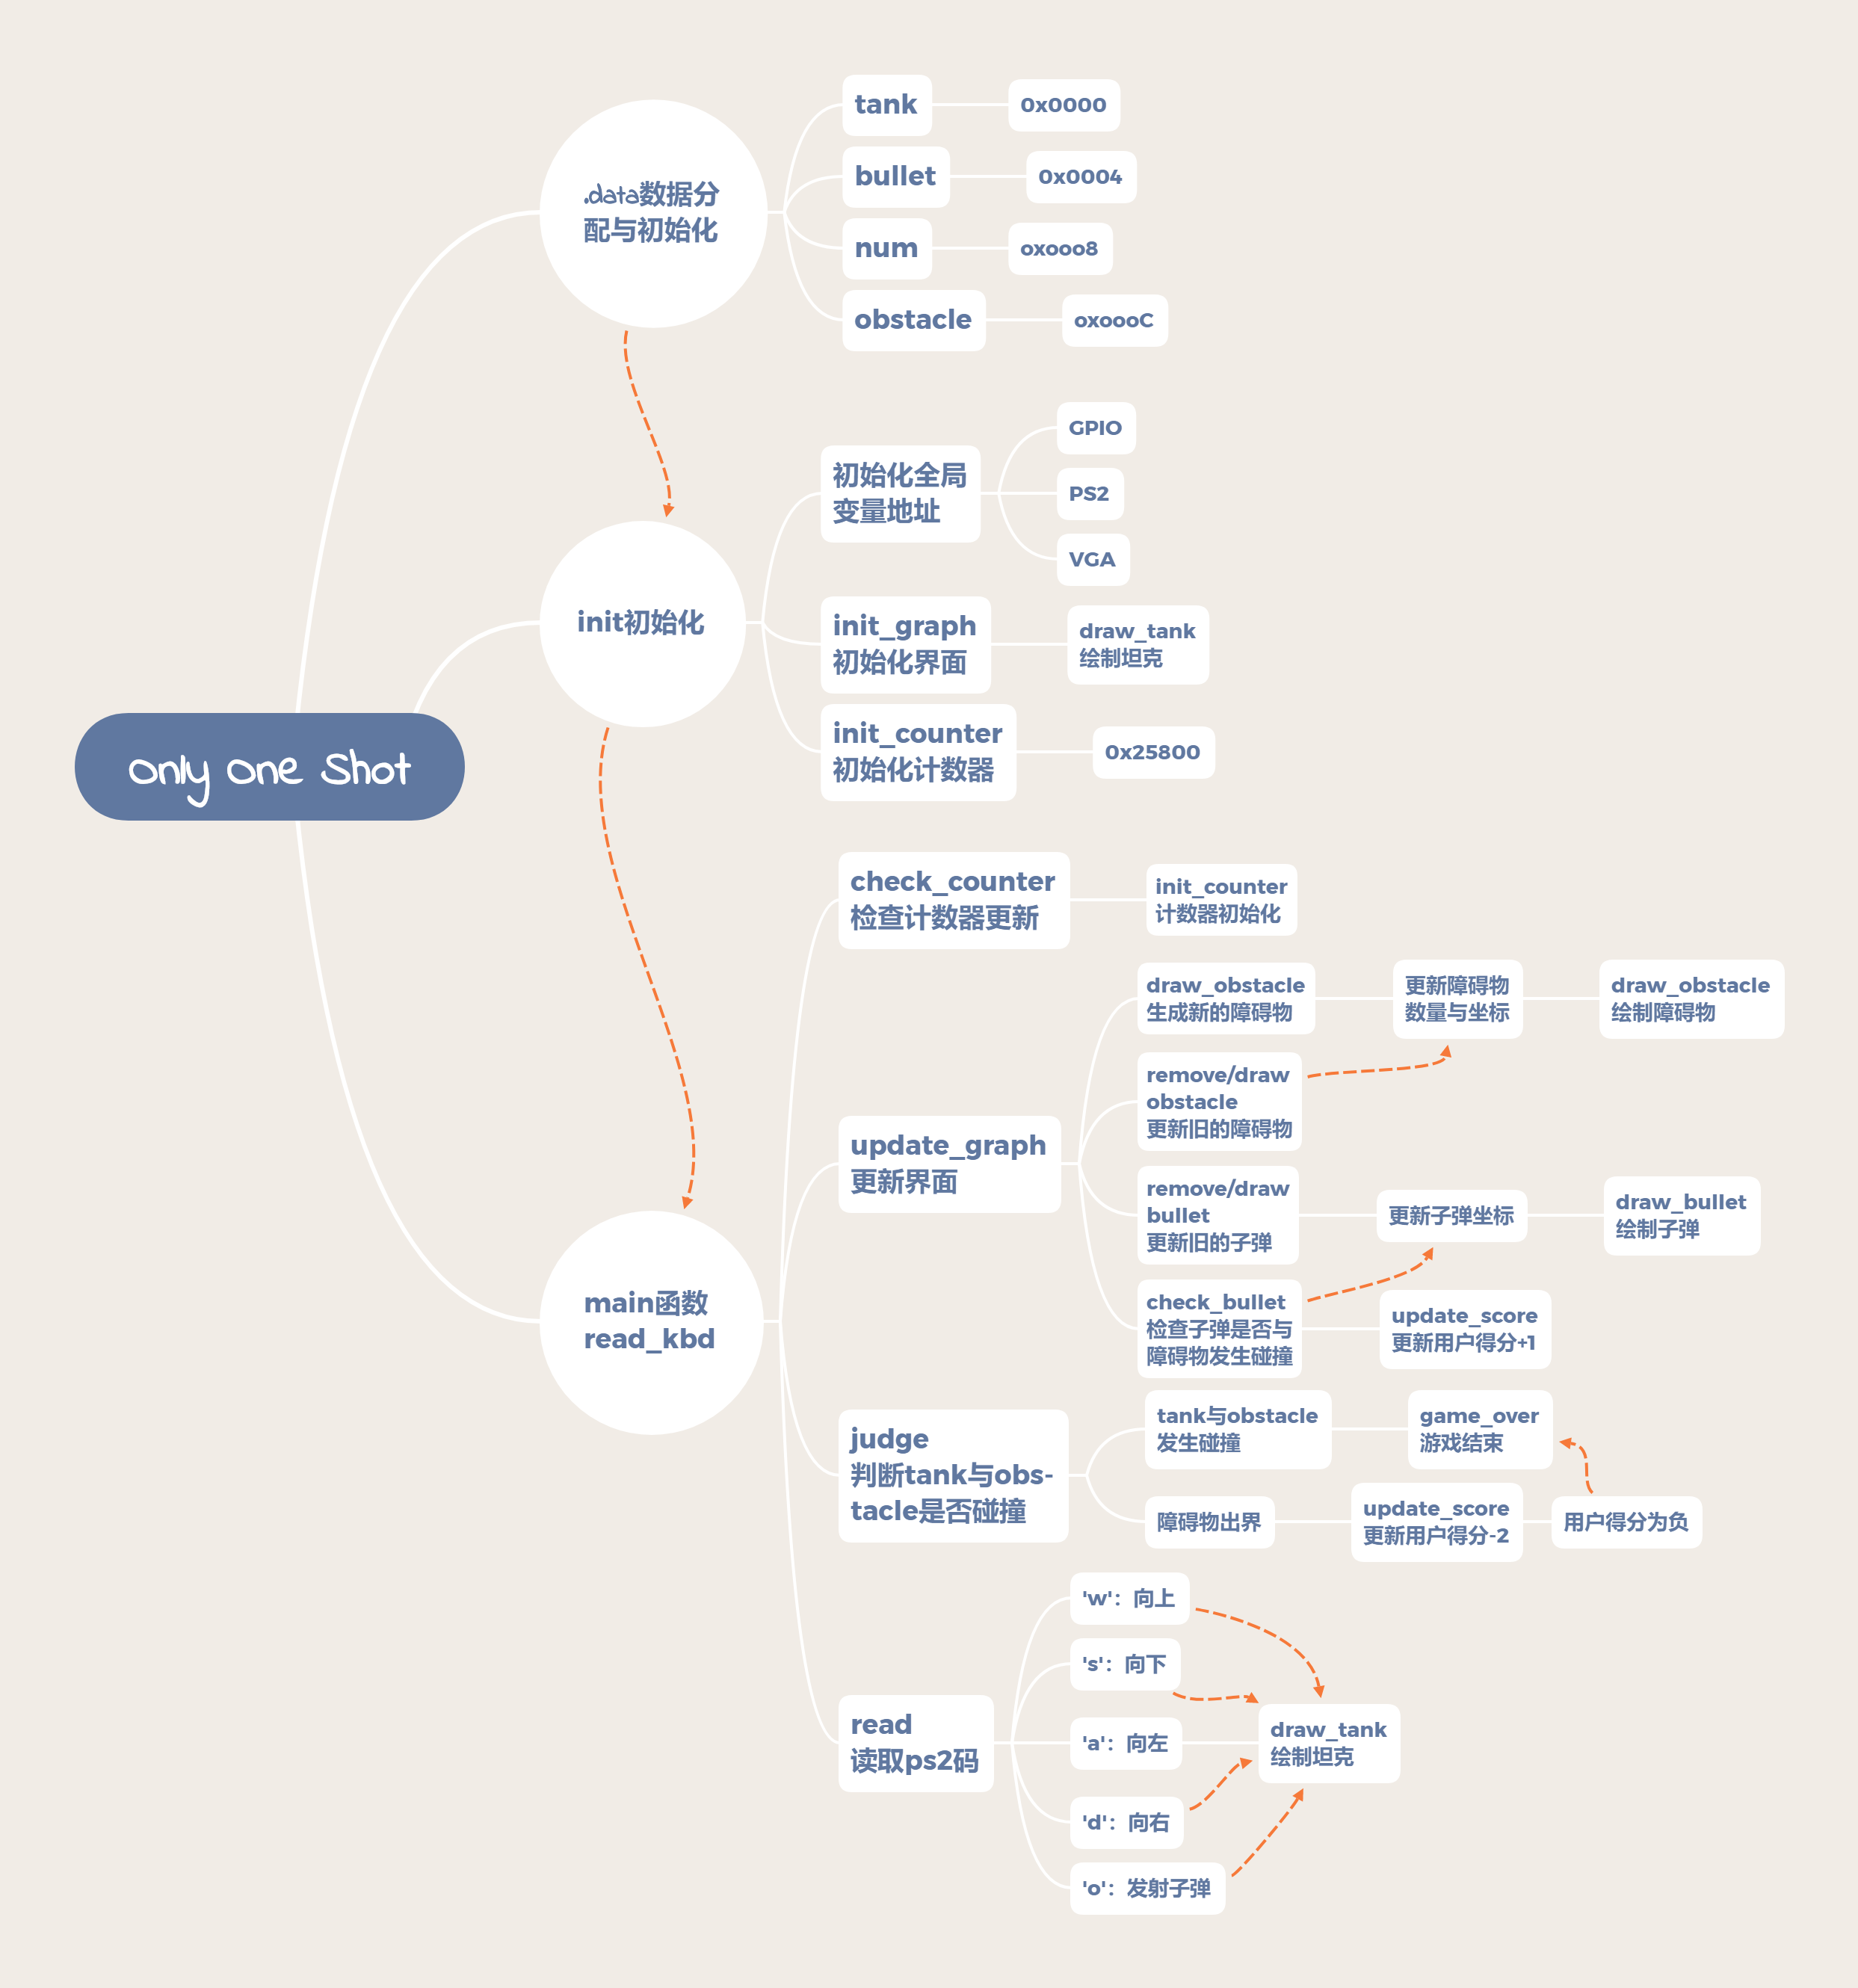
\includegraphics[width=\textwidth]{img/only-one-shot.png}
  \caption{模块概览图
  }\label{fig:modules}
\end{figure}

\subsubsection{.data空间的数据分配}
\begin{lstlisting}[frame=shadowbox] 
.data 0x00
tank:       .word   0x0     # 记录tank的(x,y)坐标,其中前16位是x,后16位是y   address=0x0000
bullet:     .word   0x0     # 记录bullet的(x,y)坐标,其中前16位是x,后16位是y address=0x0004
num:        .word   0x0     # 记录障碍物的个数                               address=0x0008
obstacle:   .word   0x0     # 记录障碍物的(x,y)坐标,其中前16位是x,后16位是y  address=0x000C
\end{lstlisting}

\subsubsection{init初始化模块}

\begin{lstlisting}[frame=shadowbox]
.text 0x40
init:
ori $sp, $zero, 0xFFFF      # 先给$sp一个地址,避免溢出
lui $k0, 0xFFFF             # $k0 = 0xFFFFFF00 GPIO地址
ori $k0, $k0, 0xFF00        
addi $k1, $k0, 4            # $k1 = 0xFFFFFF04 Counter地址
# li $s7, 0xFFFFD000
lui $s7, 0xFFFF             # $s7 = 0xFFFFD000 ps2地址
ori $s7, $s7, 0xD000
lui $s6, 0x000C       
ori $s6, $s6, 0x2000        # $s6 = vram_graph = 0x000C2000 vga地址
add $t8, $zero, $zero       # 当前得分初始化为0
add $t9, $zero, $zero       # flag初始化为0
jal init_graph              # 先初始化界面
jal init_counter            # 初始化计数器
\end{lstlisting}

通过该初始化程序将初始化一些全局变量:
\begin{itemize}
    \item[1)] \$k0=0xFFFFFF00 GPIO地址
    \item[2)] \$k1=0xFFFFFF04 Counter地址
    \item[3)] \$s7=0xFFFFD000 ps2地址
    \item[4)] \$s6=0x000C2000 vga地址
    \item[5)] \$sp=0x0000FFFF 堆栈指针地址
    \item[6)] \$t0=当前点地址
    \item[7)] \$s0=当前点的颜色
    \item[8)] \$t8=当前得分(每击中一个障碍物+1分,每出界一个障碍物-2分)
    \item[9)] \$t9=是否生成新的障碍物的flag, 当\$t9=0x00020000时生成新的障碍物
\end{itemize}

\subsubsection{ps2读取模块}
本模块通过一个无限循环来读取ps2的键盘输入,并根据输入的有效按键,反映到vga的实际显示上。比如,'w','s','a','d'按键分别对应坦克的上下左右移动,'o'按键则是对应着子弹的发射功能。\\

除此之外,基于无限循环loop的特性,每次调用该函数时都会先后访问计数器模块、图形显示更新模块、判断出界or碰撞模块等。因此该模块也可以被看作是本项目的\textbf{主函数}。

该模块主要分为两部分:\\

\textbf{1、键盘码读取(包含其他功能函数的调用)}
\begin{lstlisting}[frame=shadowbox]
read_kbd:
jal check_counter           # 检查计数器是否要重新赋值
jal update_graph            # 每次读取ps2前先更新一下vga画面,主要是更新障碍物的位置
jal judge                   # 判断更新完位置的障碍物是否与tank相撞
lui  $s5, 0x8000            # $s5 = 0x80000000 $s5最高位为1,用于取出ps2的ready信号
addi $s4, $zero, 0x00F0     # $s4 = 0x000000F0 ,F0是断码的标志,是所有key的倒数第二个断码
lw   $t1, 0($s7)            # $t1 = {1'ps2_ready, 23'h0, 8'key}
and  $t2, $t1, $s5          # 取出$t1最高位的ready信号放到$t2上
beq  $t2, $zero, read_kbd   # $t2=0表示没有ps2输入,此时跳回去接着读read_kbd
andi $t2, $t1, 0x00FF       # 如果ready=1,取出$t1低八位的通码
beq  $t2, $s4, read         # 如果$t2=0x00F0,则说明读到了倒数第二个断码,此时跳到read来显示键盘码
j read_kbd  
\end{lstlisting}
 
\textbf{2、断码识别,跳转按键对应模块}
\begin{lstlisting}[frame=shadowbox]
read:                       # 读入最后一个断码,也就是key的标识码
lw   $t1, 0($s7)            # $t1 = {1'ps2_ready, 23'h0, 8'key}
and  $t2, $t1, $s5          # 同理,取出ready信号
beq  $t2, $zero, read_kbd   # ready=0,则回去重新读
andi $t2, $t1, 0x00FF       # 否则,取出低八位的断码(标识码)
addi $s1, $zero, 0x1d       # $s1 = "w"
beq  $t2, $s1, up           # if $t2 == "w", then tank remove up
addi $s1, $zero, 0x1b       # $s1 = "s"
beq  $t2, $s1, down         # if $t2 == "s", then tank remove down
addi $s1, $zero, 0x1c       # $s1 = "a"
beq  $t2, $s1, left         # if $t2 == "a", then tank remove left
addi $s1, $zero, 0x23       # $s1 = "d"
beq  $t2, $s1, right        # if $t2 == "d", then tank remove right
addi $s1, $zero, 0x44       # $s1 = "o"
beq  $t2, $s1, shot         # if $t2 == "o", then tank shot ballet
j read_kbd                  # 跳回重新读取ps2
\end{lstlisting}

\subsubsection{界面初始化模块}
该模块由程序初始化运行时调用,构造画面背景、坦克的初始位置。绘制画面的基本思想是,遍历每一行和每一列,并对每一个坐标点进行像素的赋值。\\

\begin{lstlisting}[frame=shadowbox]
# 初始化界面
init_graph:
addi $sp, $sp, -4
sw   $ra, 0($sp)
add  $t0, $zero, $s6        # $t0为全局变量,是当前点的地址,初始化为第一个点的地址
add  $t1, $zero, $zero      # $t1表示当前扫描到的y坐标
add  $t2, $zero, $zero      # $t2表示当前扫描到的x坐标
loop_y_init:                # 每一行的遍历
slti $t3, $t1, 480          # 如果$t1=y>=480,则整个屏幕都已经遍历完了,结束扫描
beq  $t3, $zero, end_y_init        
add  $t2, $zero, $zero      # $t2=x重新初始化为当前行的第一个点坐标
loop_x_init:  
slti $t3, $t2, 640          # 如果$t2=x>=640,则当前行已经遍历完了,切换到下一行
beq  $t3, $zero, end_x_init
addi $s0, $zero, 0x00F0     # 给$s0颜色赋值,点为绿色,注意只有前16位才是rgb有效位
sh   $s0, 0($t0)            # 把$s0的前16位rgb放到当前点的地址上,后16位全0,不作使用
addi $t0, $t0, 2            # offset+=2,每个点占2byte
addi $t2, $t2, 1            # $t2=x++
j loop_x_init               # 继续遍历该行的剩余点
end_x_init:
addi $t1, $t1, 1            # $t1=y++
j loop_y_init               # 继续遍历下一行
end_y_init:
addi $a0, $zero, 320        # 在初始位置(320,479)绘制tank
addi $a1, $zero, 479        # $a0=x=0x0140, $a1=y=0x01df
sll  $s1, $a0, 16           # 将x=$a0放到$s1的高16位,$s1=0x01400000
or  $s1, $s1, $a1           # 将y=$a1放到$s1的低16位,$s1=0x014001df
add  $s2, $zero, $zero      # 获取存放tank坐标的内存地址$s2=0x0
sw   $s1, 0($s2)            # 将tank坐标存放在0x0的内存地址上
jal draw_tank               # 绘制tank
lw   $ra, 0($sp)
addi $sp, $sp, 4
jr   $ra                    # 遍历完成,返回地址
\end{lstlisting}

\subsubsection{计数器更新模块}
功能包括:计数器重新初始化+检查计数器是否需要重新初始化。
\begin{lstlisting}[frame=shadowbox]
# 重新初始化计数器
init_counter:
addi $t1, $zero, 600
sll  $t1, $t1, 8            # 600左移8位:0x0258->0x00025800,方便计数,中心点x范围:(20,620)
sw   $t1, 0($k1)            # 给计数器一个初始值600*4,是障碍物中心点出现的x轴范围*4
jr   $ra

# 检查计数器是否要重新赋值
check_counter:
addi $sp, $sp, -4
sw   $ra, 0($sp)
lw   $t3, 0($k0)            # 读取GPIO
lui  $t1, 0x8000     
and  $t2, $t3, $t1          # 取出GPIO端口最高位counter0_out信号
beq  $t2, $zero, continue   # 如果计数器还未计满数字,则不用重新给计数器赋值
jal init_counter            # 如果计数器已经计完一遍数字,则重新开始计数
continue:
lw   $ra, 0($sp)
addi $sp, $sp, 4
jr $ra
\end{lstlisting}

\subsubsection{四边形的绘制和擦除模块}
功能:画一个长方形(只会改变这个长方形范围内的像素值)。\\
input: (\$a0,\$a1)=左上角坐标, (\$a2,\$a3)=右下角坐标。\\
input: \$s0=长方形颜色。\\

\begin{lstlisting}[frame=shadowbox]
draw_rectangle:
addi $sp, $sp, -8
sw   $t3, 4($sp)
sw   $ra, 0($sp)
add  $t0, $zero, $s6        # $t0表示当前点的地址,初始化为第一个点的地址
add  $t1, $zero, $zero      # $t1表示当前扫描到的y坐标
add  $t2, $zero, $zero      # $t2表示当前扫描到的x坐标
loop_y_rec:                 # 每一行的遍历
slti $t3, $t1, 480          # 如果$t1=y>=480,则整个屏幕都已经遍历完了,结束扫描
beq  $t3, $zero, end_y_rec        
add  $t2, $zero, $zero      # $t2=x重新初始化为当前行的第一个点坐标
loop_x_rec:  
slti $t3, $t2, 640          # 如果$t2=x>=640,则当前行已经遍历完了,切换到下一行
beq  $t3, $zero, end_x_rec
slt  $t3, $t2, $a0          # 如果x的范围不在矩形框内,则直接x++
bne  $t3, $zero, jump_x_rec
slt  $t3, $a2, $t2
bne  $t3, $zero, jump_x_rec
slt  $t3, $t1, $a1          # 如果y的范围不在矩形框内,则直接x++(放在这个循环内是为了让offset也得到更新)
bne  $t3, $zero, jump_x_rec
slt  $t3, $a3, $t1
bne  $t3, $zero, jump_x_rec
sh   $s0, 0($t0)            # 把$s0的前16位rgb放到当前点的地址上,后16位全0,不作使用
jump_x_rec:
addi $t0, $t0, 2            # offset+=2,每个点占2byte
addi $t2, $t2, 1            # $t2=x++
j loop_x_rec                # 继续遍历该行的剩余点
end_x_rec:                  # 该行遍历结束
addi $t1, $t1, 1            # $t1=y++
j loop_y_rec                # 继续遍历下一行
end_y_rec:                  # 所有行遍历结束
lw   $ra, 0($sp)
lw   $t3, 4($sp)
addi $sp, $sp, 8
jr $ra
\end{lstlisting}

注:对擦除函数来说,只会改变这个四边形范围内的像素值,本质上就是把这个四边形重新赋值为背景色,因此函数内容与绘制函数基本一致,这里不再重复列出。\\

\subsubsection{坦克绘制和擦除模块}
功能: 绘制tank,实际上就是调用四边形绘制模块,用几个四边形拼接出坦克的形状。\\
input: \$a0=x, \$a1=y, 其中(x,y)为tank最下方中心点位置。\\
注意:需要保护变量\$s1, \$s2,擦除模块同理。\\

\begin{lstlisting}[frame=shadowbox]
draw_tank:
addi $sp, $sp, -20
sw   $s1, 16($sp)
sw   $s2, 12($sp)
sw   $a0, 8($sp)
sw   $a1, 4($sp)
sw   $ra, 0($sp)
add  $s1, $a1, $zero        # 保存input的(x,y)信息
add  $s2, $a0, $zero
addi $s0, $zero, 0x0F00     # tank为红色
addi $a0, $s2, -30          # tank body: (x-30,y-20)~(x+30,y)
addi $a1, $s1, -20
addi $a2, $s2, 30
add  $a3, $s1, $zero 
jal draw_rectangle          # 绘制tank body
addi $a0, $s2, -10          # tank head: (x-10,y-40)~(x+10,y-20)
addi $a1, $s1, -40
addi $a2, $s2, 10
addi $a3, $s1, -20
jal draw_rectangle          # 绘制tank head
lw   $ra, 0($sp)
lw   $a1, 4($sp)
lw   $a0, 8($sp)
lw   $s2, 12($sp)
lw   $s1, 16($sp)
addi $sp, $sp, 20
jr $ra
\end{lstlisting}

\subsubsection{子弹绘制和擦除模块}
功能: 绘制bullet,子弹是一个边长为10的正方形。\\
input: \$a0=x, \$a1=y, 其中(x,y)为obstacle最下方中心点位置\\
注意:需要保护变量\$s1, \$s2,擦除模块同理。\\

\begin{lstlisting}[frame=shadowbox]
draw_bullet:
addi $sp, $sp, -20
sw   $s1, 16($sp)
sw   $s2, 12($sp)
sw   $a0, 8($sp)
sw   $a1, 4($sp)
sw   $ra, 0($sp)
add  $s1, $a1, $zero        # 保存input的(x,y)信息到($s2,$s1)
add  $s2, $a0, $zero 
addi $s0, $zero, 0x0F00     # bullet为红色
addi $a0, $s2, -5           # 左上角($s2-5,$s1-10)
addi $a1, $s1, -10
addi $a2, $s2, 5            # 右下角($s2+5,$s1)
addi $a3, $s1, 0
jal draw_rectangle
lw   $ra, 0($sp)
lw   $a1, 4($sp)
lw   $a0, 8($sp)
lw   $s2, 12($sp)
lw   $s1, 16($sp)
addi $sp, $sp, 20
jr $ra
\end{lstlisting}

\subsubsection{障碍物绘制和擦除模块}
功能: 绘制/擦除障碍物,障碍物为边长为40的正方形。\\
input: \$a0=x, \$a1=y, 其中(x,y)为obstacle最上方中心点位置。\\
注意:需要保护变量\$s1, \$s2,擦除模块同理。\\

\begin{lstlisting}[frame=shadowbox]
draw_obstacle:
addi $sp, $sp, -20
sw   $s1, 16($sp)
sw   $s2, 12($sp)
sw   $a0, 8($sp)
sw   $a1, 4($sp)
sw   $ra, 0($sp)
add  $s1, $a1, $zero        # 保存input的(x,y)信息到($s2,$s1)
add  $s2, $a0, $zero 
addi $s0, $zero, 0x000F     # obstacle为蓝色
addi $a0, $s2, -20          # 左上角($s2-20,$s1)
add  $a1, $s1, $zero
addi $a2, $s2, 20           # 右下角($s2+20,$s1+40)
addi $a3, $s1, 40
jal draw_rectangle
lw   $ra, 0($sp)
lw   $a1, 4($sp)
lw   $a0, 8($sp)
lw   $s2, 12($sp)
lw   $s1, 16($sp)
addi $sp, $sp, 20
jr $ra
\end{lstlisting}

\subsubsection{坐标与地址转换模块}
该模块用于空间坐标与实际地址的相互转化,方便根据坐标对对应点的像素值进行读写操作。\\
功能: 将输入的x,y坐标转化为实际地址。\\
input: (x=\$a0,y=\$a1)。\\
output: \$v0=address。\\

\begin{lstlisting}[frame=shadowbox]
coordinate_to_address:
addi $sp, $sp, -16
sw   $t0, 12($sp)
sw   $t3, 8($sp)
sw   $t1, 4($sp)
sw   $ra, 0($sp)
add  $t0, $zero, $s6        # $t0是当前点的地址,初始化为第一个点的地址
add  $t1, $zero, $zero      # $t1=y=0
loop_y:
slt  $t3, $t1, $a1 
beq  $t3, $zero, end_y
addi $t0, $t0, 1280         # 640*2=1280 每一行640个点,每个点2byte,即更新$t0为下一行第一个点的位置
addi $t1, $t1, 1            # $t1=y++
j loop_y
end_y:
add  $t0, $t0, $a0          # offset_x=2*x
add  $t0, $t0, $a0          # $t0已经是(x,y)点的实际地址
add  $v0, $t0, $zero
lw   $ra, 0($sp)
lw   $t1, 4($sp)
lw   $t3, 8($sp)
lw   $t0, 12($sp)
addi $sp, $sp, 16
jr   $ra
\end{lstlisting}

\subsubsection{界面更新模块}
该模块为整个程序中\textbf{最为重要的模块},所显示出来的物体移动效果实际上都是通过该模块的坐标修改、重新绘制并刷新界面得到的。
该模块主要分为以下几个部分:\\

\textbf{1、通过flag判断是否生成障碍物}\\
如果flag!=20,则只更新旧的障碍物,不生成新的障碍物;如果flag=20,则生成新的障碍物,且\$t9=flag清零,此时读取counter并将之转化为新生成障碍物的坐标。\\

\begin{lstlisting}[frame=shadowbox]
update_graph:
addi $sp, $sp, -4
sw   $ra, 0($sp)
addi $t9, $t9, 1            # $t9=flag++
addi $t1, $zero, 20          
bne  $t9, $t1, update_old   # 如果flag!=20,则只更新旧的障碍物,不生成新的障碍物
add  $t9, $zero, $zero      # 如果flag=20,则生成新的障碍物,且$t9=flag清零
lw   $t1, 0($k1)            # 范围:0x00000000~0x00025800
srl  $t1, $t1, 8            # 右移8bit:0x0000~0x0258<=>(0,600)
addi $t1, $t1, 20           # 获取随机生成的障碍物中心点x坐标(20,620)
...
update_old:
...
lw   $ra, 0($sp)
addi $sp, $sp, 4
jr $ra
\end{lstlisting}

\textbf{2、将新生成的obstacle插入障碍物数组并绘制}\\
如果生成新的障碍物,则要执行这一过程。注意,新生成的障碍物坐标用一个word存储,x坐标放入寄存器的高16位,y坐标则放入寄存器的低16位。插入的时候,新的元素插入数组头,旧的元素往数组尾挪动一个word。这样做有一个好处是,当最旧的元素出界时,直接从数组尾部移除即可,无需再挪动其他元素在内存的位置。\\

\begin{lstlisting}[frame=shadowbox]
# ------------------将新生成的obstacle插入障碍物数组 begin-----------------------
sll  $s1, $t1, 16           # 将($t1,0)压缩到一个寄存器$s1里,x为高16位,y为低16位
addi $s2, $zero, 0x0008     # 获取存放障碍物个数num的内存地址
lw   $s3, 0($s2)            # 获取当前的障碍物个数$s3=num
addi $s3, $s3, 1            # 障碍物个数num++
sw   $s3, 0($s2)            # 更新num
addi $s2, $zero, 0x000C     # 获取存放障碍物坐标数组头的内存地址$s2
addi $s3, $s3, -1           # $s3=$s3-1
insert_obs:                 # 寻找存放新增的障碍物(x,y)坐标的内存地址,更新到$s2
beq  $s3, $zero, end_insert_obs
lw   $s4, 0($s2)            # 保存当前扫描到的障碍物坐标到$s4
sw   $s1, 0($s2)            # 将上一个障碍物的坐标$s1存到当前位置上
add  $s1, $zero, $s4        # 更新上一个障碍物的坐标$s1=$s4
addi $s2, $s2, 4
addi $s3, $s3, -1
j insert_obs
end_insert_obs:             # 更新最后一个障碍物坐标的位置,插入完毕后,绘制该障碍物
sw   $s1, 0($s2)            # 将上一个障碍物的坐标$s1存到当前位置上
add  $a0, $t1, $zero        # ($t1,0)
add  $a1, $zero, $zero
addi $s0, $zero, 0x000F     # 设置障碍物为蓝色
jal draw_obstacle           # 绘制障碍物
# -----------------将新生成的obstacle插入障碍物数组 end---------------------------
\end{lstlisting}

\textbf{3、刷新所有已经存在的子弹的位置并绘制}\\
由于障碍物和子弹一旦生成,就会以一定速度往既定方向移动,这个部分就是用于更新子弹的坐标并刷新显示的。需要额外注意的是,在子弹移动的过程中,一旦与某个障碍物发生碰撞,则需要在画面上同时移除子弹和对应的障碍物,以显示出击中的效果。\\

\begin{lstlisting}[frame=shadowbox]
# ---------------------------update bullet----------------------------------
#update_bullet:
addi $s2, $zero, 0x0004     # 取出bullet坐标地址
lw   $s1, 0($s2)            # bullet的(x,y)坐标,赋给$s1
beq  $s1, $zero, update_obs # 如果bullet坐标为0,则要么是初始状态,要么已经发生碰撞,需要再次按下'o'才能触发新的bullet
lui  $a0, 0xFFFF            # 提取出x坐标赋给$a0
and  $a0, $a0, $s1
srl  $a0, $a0, 16
ori  $a1, $zero, 0xFFFF     
and  $a1, $a1, $s1          # 提取出y坐标赋给$a1
jal remove_bullet           # 移除bullet
addi $a1, $a1, -5           # x坐标不变,更新y坐标$a1=y-5
jal draw_bullet             # 重新绘制bullet,以显示移动的效果
sll $s1, $a0, 16
or  $s1, $s1, $a1           # 把该障碍物新的坐标重新赋给$s1
addi $a1, $a1, -10          # 获取bullet头部中心点的y坐标
jal check_bullet            # 判断是否与障碍物碰撞
beq $v0, $zero, no_bullet_collision
add  $s1, $zero, $zero      # 如果发生碰撞,则bullet坐标清零
addi $a1, $a1, 10           # 恢复刚刚画的bullet的坐标
jal remove_bullet           # 移除刚刚画的bullet
# ----------------------------update score and max_score---------------------
addi $a0, $zero, 1
jal update_score
# --------------------------------------------------------------------------
no_bullet_collision:
sw  $s1, 0($s2)             # 将$s1重新存储到指定内存地址
# --------------------------------------------------------------------------
\end{lstlisting}

\textbf{4、刷新所有已经存在的障碍物的位置并绘制}\\
原理与子弹更新部分相同。\\

\begin{lstlisting}[frame=shadowbox]
# ---------------------------update obstacle--------------------------------
update_obs:
addi $s2, $zero, 0x0008     # 获取存放障碍物个数num的内存地址
lw   $s3, 0($s2)            # 获取当前的障碍物个数$s3=num
addi $s2, $zero, 0x000C     # 获取存放障碍物坐标数组头的内存地址$s2
traverse_obs_addr:
beq  $s3, $zero, end_traverse
lw   $s1, 0($s2)            # 遍历每一个obstacle的(x,y)坐标,赋给$s1
lui  $a0, 0xFFFF            # 提取出x坐标赋给$a0
and  $a0, $a0, $s1
srl  $a0, $a0, 16
ori  $a1, $zero, 0xFFFF     # 注意,addi是有符号位扩展,addi $a1, $zero, 0xFFFF是错误的!应当使用ori
and  $a1, $a1, $s1          # 提取出y坐标赋给$a1
jal remove_obstacle         # 移除障碍物
addi $a1, $a1, 5            # x坐标不变,更新y坐标$a1=y+5
jal draw_obstacle           # 重新绘制障碍物,以显示移动的效果
sll $s1, $a0, 16
or  $s1, $s1, $a1           # 把该障碍物新的坐标重新赋给$s1
sw  $s1, 0($s2)             # 将$s1重新存储到指定内存地址
addi $s2, $s2, 4            # 下一个障碍物的地址
addi $s3, $s3, -1           # num--
j traverse_obs_addr
end_traverse:
# ------------------------------------------------------------------------------
\end{lstlisting}

\subsubsection{分数更新模块}
该模块用于更新用户已获得的分数,以及历史最高分数。如果当前用户分数为负,则游戏结束。\\
input: \$a0=+1(击中障碍物+1) or \$a0=0(障碍物出界-2)\\

\begin{lstlisting}[frame=shadowbox]
update_score:
addi $sp, $sp, -20
sw   $t3, 16($sp)
sw   $s1, 12($sp)
sw   $s2, 8($sp)
sw   $s3, 4($sp)
sw   $ra, 0($sp)
beq  $a0, $zero, minus_score
addi $t8, $t8, 1 
j read_score
minus_score:
slti $t3, $t8, 2            # 如果$t8小于2,则obstacle出界后得分为负,游戏结束
beq  $t3, $zero, minus_con
j game_over
minus_con:
addi $t8, $t8, -2
read_score:
lui  $s1, 0xFFFF
ori  $s1, $s1, 0xFE00       # $t1=七段数码管地址=0xFFFFFE00
lw   $s2, 0($s1)            # 读取显示的数据,前4个数码管为max_score,后4个数码管为当前score
srl  $s2, $s2, 16 
slt  $s3, $s2, $t8          # 判断是否要更新max score
beq  $s3, $zero, update_r_score
sll  $s2, $t8, 16
or   $s2, $s2, $t8
j update_all_score
update_r_score:
sll  $s2, $s2, 16
or   $s2, $s2, $t8
update_all_score:
sw   $s2, 0($s1)            # 将当前得分更新到七段数码管显示
lw   $ra, 0($sp)
lw   $s3, 4($sp)
lw   $s2, 8($sp)
lw   $s1, 12($sp)
lw   $t3, 16($sp)
addi $sp, $sp, 20
jr   $ra
\end{lstlisting}

\subsubsection{判断坦克是否会与障碍物发生碰撞}
这里通过检测坦克上表面点的上方像素点的颜色来判定。\\
1、判断tank是否会与障碍物发生碰撞,如果发生碰撞,则游戏重新开始。\\
2、判断障碍物是否超出界面,如果超出边界,则清空对应地址上的坐标,且障碍物个数-1。\\

\begin{lstlisting}[frame=shadowbox]
judge:
addi $sp, $sp, -4
sw   $ra, 0($sp)
addi $s2, $zero, 0x0000
lw   $s1, 0($s2)            # 取出tank的坐标
lui  $a0, 0xFFFF            # 获取tank的x坐标
and  $a0, $a0, $s1
srl  $a0, $a0, 16 
ori  $a1, $zero, 0xFFFF
and  $a1, $a1, $s1          # 获取tank下边界中心点的y坐标
addi $a1, $a1, -41          # 获取tank上边界上一行中心点的y坐标
jal coordinate_to_address
addi $t1, $zero, 0x000F     # 蓝色
lh   $s0, 0($v0)            
bne  $s0, $t1, judge_tank_left 
j game_over
judge_tank_left:
addi $a0, $a0, -30
addi $a1, $a1, 20
jal coordinate_to_address
addi $t1, $zero, 0x000F     # 蓝色
lh   $s0, 0($v0)            
bne  $s0, $t1, judge_tank_right 
j game_over
judge_tank_right:
addi $a0, $a0, 60
jal coordinate_to_address
addi $t1, $zero, 0x000F     # 蓝色
lh   $s0, 0($v0)            
bne  $s0, $t1, judge_obs_traversal 
j game_over
judge_obs_traversal:
addi $s2, $zero, 0x0008     # 获取存放障碍物个数num的内存地址
lw   $s3, 0($s2)            # 获取当前的障碍物个数$s3=num
add  $t3, $zero, $s3        # 用$t3保存当前还剩余的障碍物个数,初始化为num
addi $s2, $zero, 0x000C     # 获取存放障碍物坐标数组头的内存地址$s2
judge_obs:
beq  $s3, $zero, end_judge
lw   $s1, 0($s2)            # 遍历每一个obstacle的(x,y)坐标,赋给$s1
ori  $t1, $zero, 0xFFFF
and  $t1, $s1, $t1          # 获取obstacle上边界中心点的y坐标,赋给$t1,
judge_edge:
slti $t2, $t1, 479
bne  $t2, $zero, judge_next # 如果还未到达边界,则继续遍历下一个obstacle
sw   $zero, 0($s2)          # 如果到达边界,则当前扫描到的地址赋值为0
addi $t3, $t3, -1           # 当前剩余的障碍物个数-1 
add  $a0, $zero, $zero      # 障碍物出界,得分-2
jal update_score
judge_next:
addi $s2, $s2, 4            # 下一个障碍物的地址
addi $s3, $s3, -1           # num--
j judge_obs
end_judge:
addi $s2, $zero, 0x0008     # 获取存放障碍物个数num的内存地址
sw   $t3, 0($s2)            # 更新当前的障碍物个数为$t3
lw   $ra, 0($sp)
addi $sp, $sp, 4
jr $ra
\end{lstlisting}

\subsubsection{判断子弹是否会与障碍物发生碰撞}
功能: 判断bullet是否会与障碍物撞上,这里通过检测子弹上边界的上一行的颜色来判定。\\
input: \$a0=x, \$a1=y (默认是子弹上边界中心点坐标)\\
output: \$v0=1: 已经碰撞,\$v0=0: 尚未碰撞\\

\begin{lstlisting}[frame=shadowbox]
check_bullet:
addi $sp, $sp, -20
sw   $s1, 16($sp)
sw   $s2, 12($sp)
sw   $a0, 8($sp)
sw   $a1, 4($sp)
sw   $ra, 0($sp)
addi $a1, $a1, -1           # 取出上一行点的y坐标
add  $t6, $zero, $a1        # 保存该y坐标到$t6
jal coordinate_to_address
lh   $t1, 0($v0)            # 取出上一行点的rgb
#add  $gp, $zero, $t1
addi $t2, $zero, 0x000F     # 与障碍物的蓝色对比
addi $v0, $zero, 0
bne  $t1, $t2, check_end
addi $v0, $zero, 1
addi $s2, $zero, 0x0008     # 获取存放障碍物个数num的内存地址
lw   $s3, 0($s2)            # 获取当前的障碍物个数$s3=num
add  $t3, $zero, $s3        # 用$t3保存当前还剩余的障碍物个数,初始化为num
addi $s2, $zero, 0x000C     # 获取存放障碍物坐标数组头的内存地址$s2
add  $t5, $zero, $zero      # flag=0
check_obs:
beq  $s3, $zero, check_obs_end
lw   $s1, 0($s2)            # 遍历每一个obstacle的(x,y)坐标,赋给$s1
beq  $t5, $zero, check_obs_con
addi $t2, $s2, -4           # 如果$t5=flag=1,则将当前坐标上移一个byte
sw   $s1, 0($t2)
sw   $zero, 0($s2)          # 当前地址上的坐标清空
j check_bos_next
check_obs_con:
lui  $a0, 0xFFFF            # 提取出x坐标赋给$a0
and  $a0, $a0, $s1
srl  $a0, $a0, 16
ori  $a1, $zero, 0xFFFF
and  $a1, $s1, $a1          # 提取出y坐标赋给$a1
add  $t1, $zero, $a1        # 获取obstacle的y坐标上界$t1
addi $t2, $t1, 40           # 获取obstacle的y坐标下界$t2
slt  $t4, $t6, $t2
beq  $t4, $zero, check_bos_next
slt  $t4, $t1, $t6
beq  $t4, $zero, check_bos_next
addi $t5, $zero, 1
addi $t3, $t3, -1
jal remove_obstacle
check_bos_next:
addi $s2, $s2, 4            # 下一个障碍物的地址
addi $s3, $s3, -1           # num--
j check_obs
check_obs_end:
addi $s2, $zero, 0x0008     # 获取存放障碍物个数num的内存地址
sw   $t3, 0($s2)            # 更新当前的障碍物个数为$t3
check_end:
lw   $ra, 0($sp)
lw   $a1, 4($sp)
lw   $a0, 8($sp)
lw   $s2, 12($sp)
lw   $s1, 16($sp)
addi $sp, $sp, 20
jr   $ra
\end{lstlisting}

\subsubsection{坦克的上下左右移动}
由于上下左右移动的函数大致相同,因此这里只展示向上移动的函数内容。\\

\begin{lstlisting}[frame=shadowbox]
up:
addi $sp, $sp, -20
sw   $s1, 16($sp)
sw   $s2, 12($sp)
sw   $a0, 8($sp)
sw   $a1, 4($sp)
sw   $ra, 0($sp)
addi $s2, $zero, 0x0000     # 存放tank地址的内存空间
lw   $s1, 0($s2)            # 取出tank地址
lui  $a0, 0xFFFF            # 提取出x坐标赋给$a0
and  $a0, $a0, $s1
srl  $a0, $a0, 16
ori  $a1, $zero, 0xFFFF     # 提取出y坐标赋给$a1 
and  $a1, $a1, $s1          
jal  remove_tank
addi $a1, $a1, -20          # tank坐标上移20
jal  draw_tank
sll  $s1, $a0, 16
or   $s1, $s1, $a1
sw   $s1, 0($s2)            # 把新的tank坐标存放到指定内存地址
lw   $ra, 0($sp)
lw   $a1, 4($sp)
lw   $a0, 8($sp)
lw   $s2, 12($sp)
lw   $s1, 16($sp)
addi $sp, $sp, 20
jr $ra
\end{lstlisting}

\subsubsection{子弹发射}
用户按下按键'o',便可触发该函数,子弹发射的初始位置为坦克的尾部,在发射出去之前,会有一个出膛的动画演示过程。\\

\begin{lstlisting}[frame=shadowbox]
shot:
addi $sp, $sp, -20
sw   $s1, 16($sp)
sw   $s2, 12($sp)
sw   $a0, 8($sp)
sw   $a1, 4($sp)
sw   $ra, 0($sp)
addi $s2, $zero, 0x0004     # 获取存放bullet坐标的内存地址
lw   $s1, 0($s2)            # 取出bullet坐标
lui  $a0, 0xFFFF            # 提取出x坐标赋给$a0
and  $a0, $a0, $s1
srl  $a0, $a0, 16
ori  $a1, $zero, 0xFFFF     # 提取出y坐标赋给$a1
and  $a1, $a1, $s1
jal remove_bullet           # 删去原先已经发射的bullet
addi $s2, $zero, 0x0000     # 获取存放tank坐标的内存地址
lw   $s1, 0($s2)            # 取出tank坐标
lui  $a0, 0xFFFF            # 提取出x坐标赋给$a0
and  $a0, $a0, $s1
srl  $a0, $a0, 16
ori  $a1, $zero, 0xFFFF     # 提取出y坐标赋给$a1
and  $a1, $a1, $s1
#addi $a1, $a1, -40
sll  $s1, $a0, 16           # 重新合成bullet的坐标放到$s1里
or   $s1, $s1, $a1
addi $s2, $zero, 0x0004     # 获取存放bullet坐标的内存地址
sw   $s1, 0($s2)            # 将新的bullet坐标存放到指定内存地址
jal draw_bullet
lw   $ra, 0($sp)
lw   $a1, 4($sp)
lw   $a0, 8($sp)
lw   $s2, 12($sp)
lw   $s1, 16($sp)
addi $sp, $sp, 20
jr $ra

\end{lstlisting}

\subsubsection{游戏结束}
清除.data区域的数据,并清除当前用户得分,重新跳转到初始化init模块\\

\begin{lstlisting}[frame=shadowbox]
game_over:
lui  $t1, 0xFFFF
ori  $s1, $t1, 0xFE00       # $s1=七段数码管地址
lw   $s2, 0($s1)            # 读取显示的数据,前4个数码管为max_score,后4个数码管为当前score
and  $s2, $s2, $t1          # 只保留最高分,最低分清零
sw   $s2, 0($s1)            # 更新score,开启下一轮
add  $s2, $zero, $zero
sw   $zero, 0($s2)          # tank坐标清零
addi $s2, $s2, 4 
sw   $zero, 0($s2)          # bullet坐标清零
addi $s2, $s2, 4
lw   $s1, 0($s2)
game_clear:                 # obstacle清零
beq  $s1, $zero, clear_end
sw   $zero, 0($s2)
addi $s2, $s2, 4
lw   $s1, 0($s2)
j game_clear
clear_end:
j init
\end{lstlisting}

